\documentclass[runningheads]{llncs}

% ---------------------------------------------------------------
% ECCV Packages
\usepackage[review,year=2026,ID=*****]{eccv}
\usepackage{eccvabbrv}
\usepackage{graphicx}
\usepackage{booktabs}
\usepackage{algorithm}
\usepackage{algorithmic}
%\usepackage[accsupp]{axessibility}
\usepackage{hyperref}
\usepackage{orcidlink}

% Math and Utilities
\usepackage{amsmath}
\usepackage{amssymb}
\usepackage{mathtools}
% \usepackage{amsthm} % llncs defines its own theorem environments
\usepackage{newtxtext,newtxmath}
\usepackage{multirow}
\usepackage{xcolor}
\usepackage{subcaption}

% Efficient cross-referencing package
\usepackage[capitalize,noabbrev]{cleveref}

\def\httilde{\mbox{\tt\raisebox{-.5ex}{\symbol{126}}}}

\begin{document}

\title{SALMA: Mask-Guided Structure-Aware Alignment for Referring Segmentation}
\titlerunning{SALMA: Mask-Guided Structure-Aware Alignment}

\author{Your Name\inst{1} \and
Second Author\inst{2}}
\authorrunning{Y. Name et al.}
\institute{Institution Name \\
\email{first.author@i1.org} \and
Institution2 \\
\email{second.author@i2.org}}

\maketitle




%%%%%%%%% ABSTRACT
\begin{abstract}
Unified Multimodal LLMs (MLLMs) enable referring segmentation but often suffer from attention drift---erroneously attending to salient distractors rather than the queried target due to a lack of explicit spatial constraints. To bridge this semantic-structural gap, we propose \textbf{SALMA}, a novel framework that repurposes the segmentation decoder itself as a structural guide. Unlike existing methods that rely on sparse \texttt{[SEG]} tokens, SALMA introduces a Mask-Biased Attention (MBA) mechanism. Key to our innovation is a cost-effective pre-pass strategy: we leverage the frozen SAM-2 decoder to extract class-agnostic structural priors, which are then transformed into a dense soft gate to modulate the MLLM's cross-modal attention. This design effectively suppresses background noise and enforces structure-aware reasoning with negligible computational overhead ($\sim$0.7\% latency). We further enforce semantic and structural alignment using a text--mask contrastive objective and a boundary consistency loss. On Ref-DAVIS17 and Ref-YouTube-VOS, SALMA improves J\&F by +3.4 and +1.7 over Sa2VA-1B, demonstrating that stronger structural grounding can be achieved without sacrificing efficiency. Code and models will be made publicly available.
\keywords{Referring Segmentation \and Multimodal LLMs \and Spatial Alignment}
\end{abstract}

%%%%%%%%% BODY TEXT
\section{Introduction}

Unified Multimodal Large Language Models (MLLMs) have recently emerged as a powerful paradigm for visual understanding.
Frameworks like Sa2VA \cite{sa2va} and LIRA \cite{lira} integrate LLM reasoning (e.g., Qwen~\cite{qwen}, InternVL~\cite{internvl}) with the pixel-level precision of SAM-2 \cite{sam2}, aiming to enable general-purpose grounding within a single architecture.

\begin{figure*}[h!]
    \centering
    \setlength{\abovecaptionskip}{5pt}
    \setlength{\belowcaptionskip}{-5pt}
    
    % --- Row 1: Relative Position ---
    \begin{subfigure}[t]{0.32\linewidth}
        \centering
        \scriptsize \textbf{Input Image} \par \medskip
        
\includegraphics[width=1\linewidth]{figures/cup.jpg}
    \end{subfigure}
    \hfill
    \begin{subfigure}[t]{0.32\linewidth}
        \centering
        \scriptsize \textbf{OMG-LLaVA} \par \medskip
        \includegraphics[width=1\linewidth]{figures/cup_llava.jpg}
    \end{subfigure}
    \hfill
    \begin{subfigure}[t]{0.32\linewidth}
        \centering
        \scriptsize \textbf{Ours} \par \medskip
        \includegraphics[width=1\linewidth]{figures/cup_sa2va.jpg}
    \end{subfigure}
    
    \vspace{1mm}
    \begin{minipage}{0.98\linewidth}
        \centering
        \scriptsize \textit{"Segment the mug \textbf{behind} the laptop."}
    \end{minipage}
    
    \vspace{1mm}

    % --- Row 2: Spatial Ordering ---
    \begin{subfigure}[t]{0.32\linewidth}
        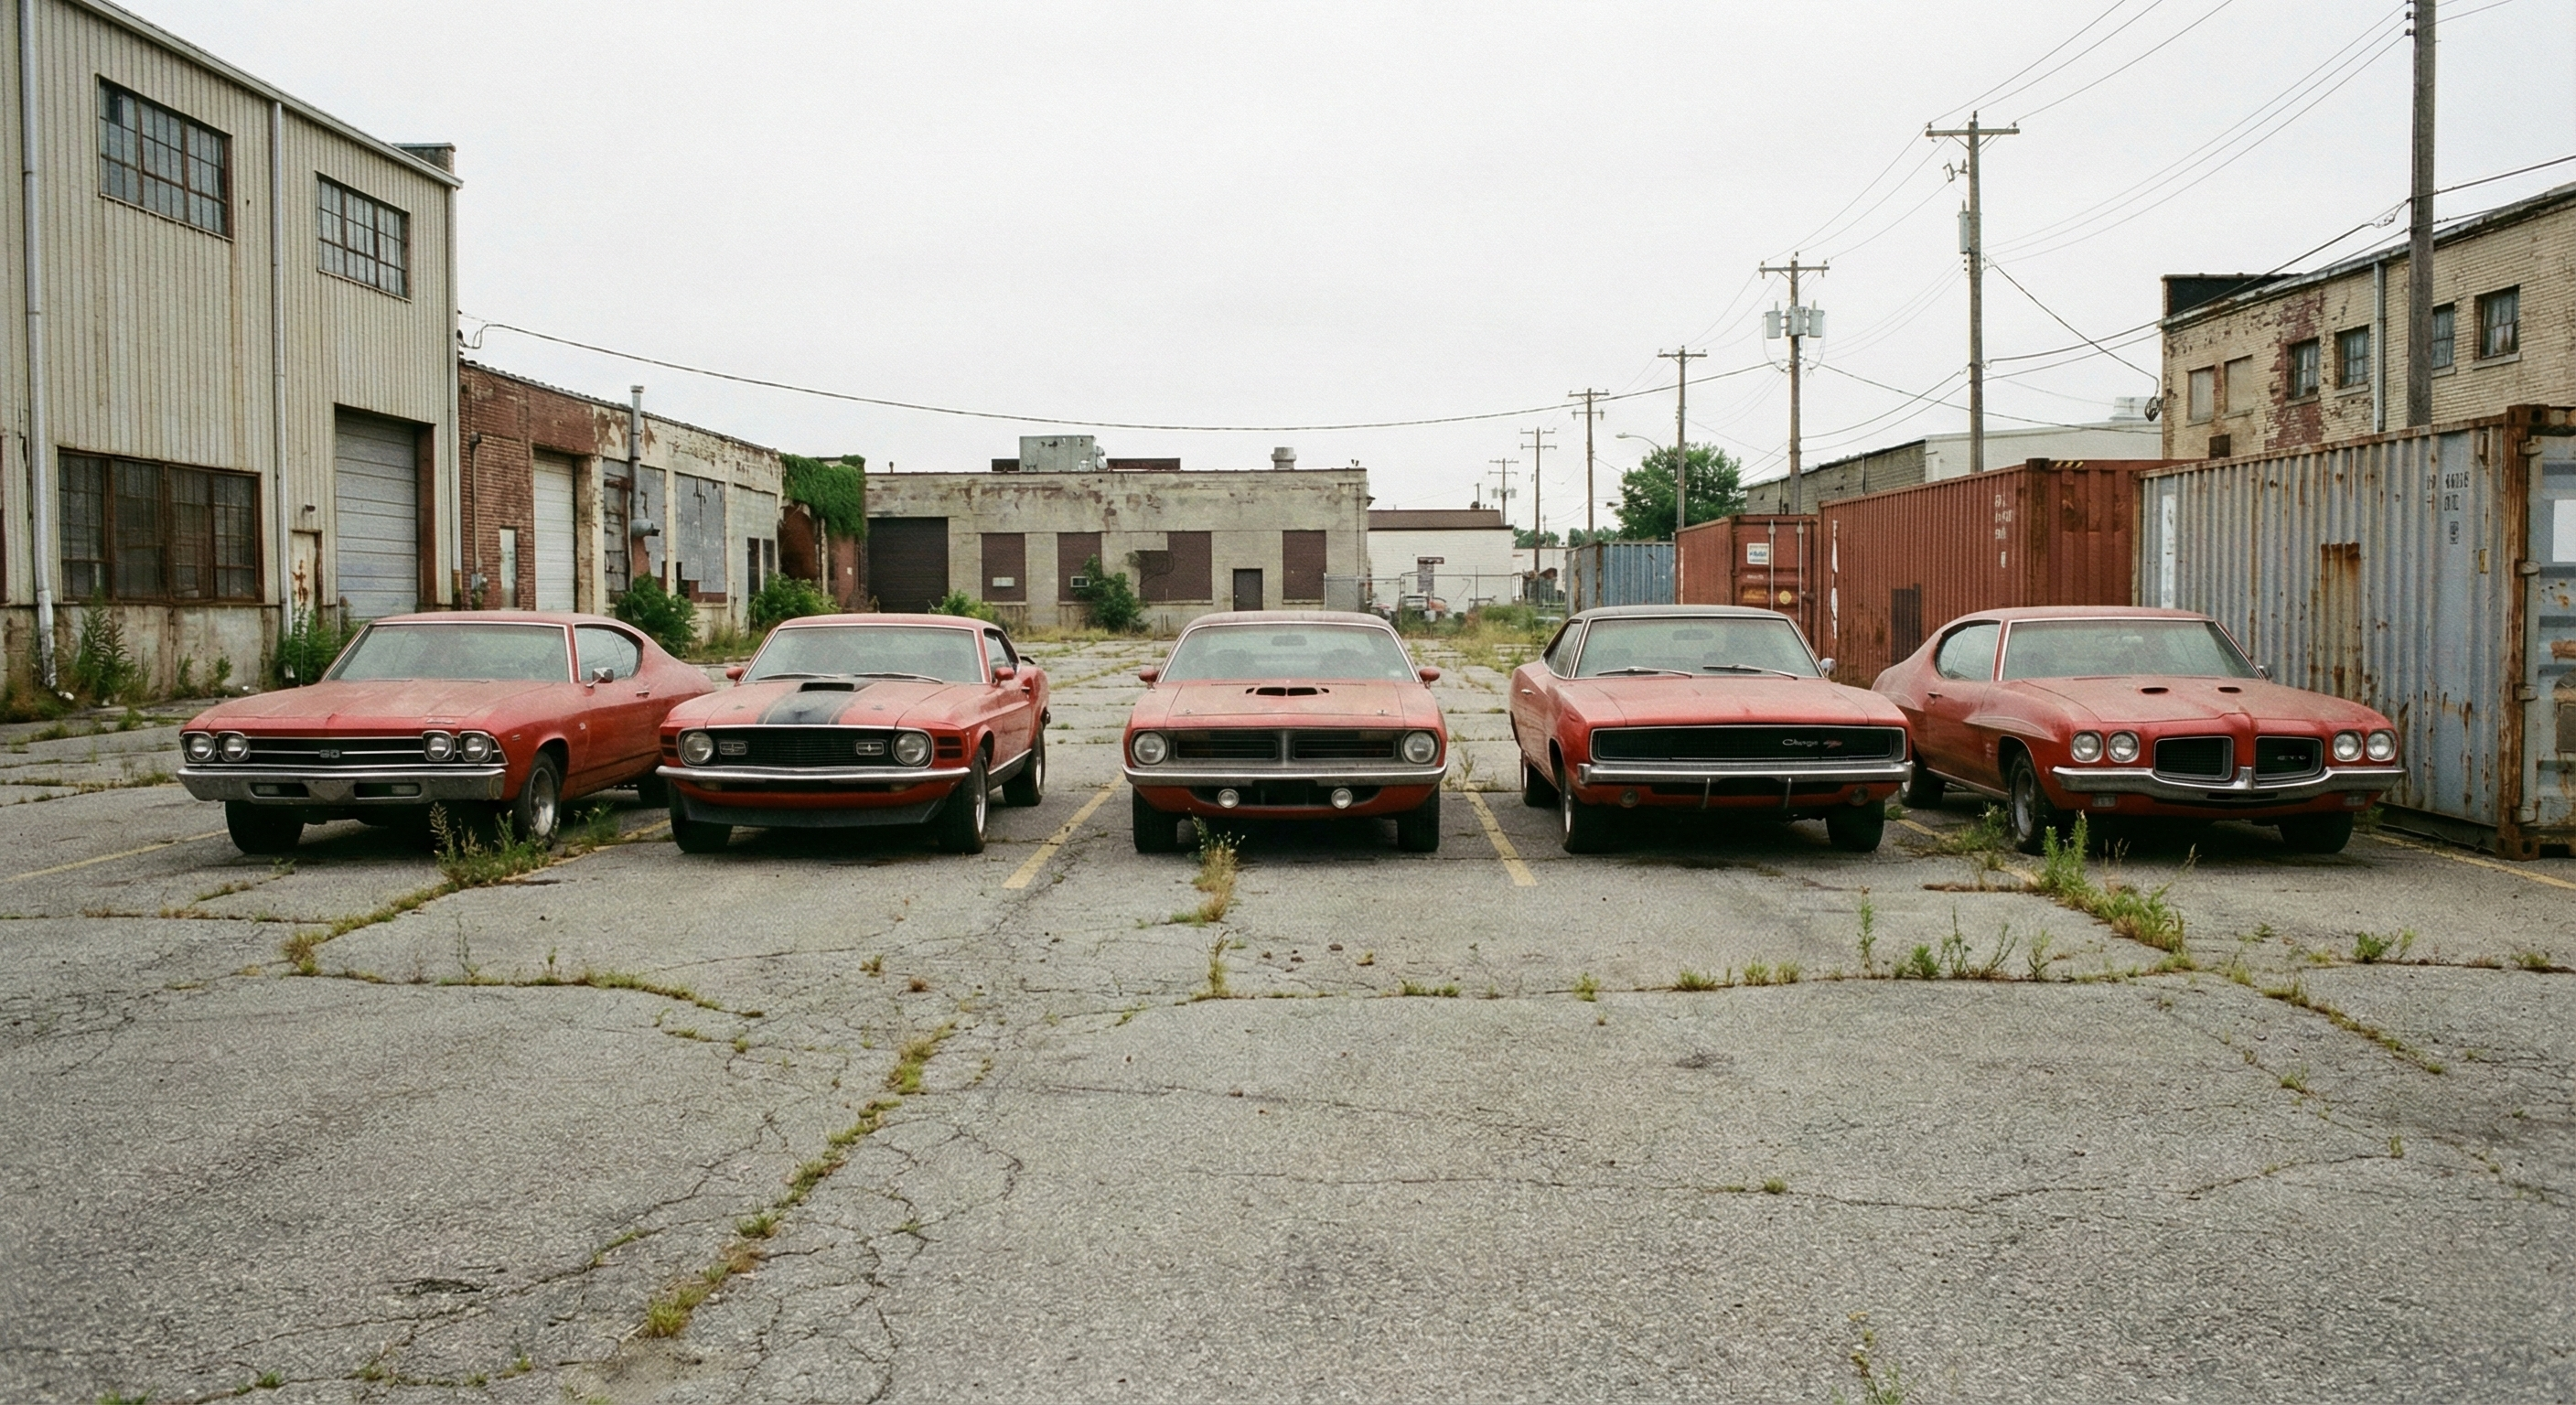
\includegraphics[width=1\linewidth]{figures/car.jpg}
    \end{subfigure}
    \hfill
    \begin{subfigure}[t]{0.32\linewidth}
        \includegraphics[width=1\linewidth]{figures/car_llava.jpg}
    \end{subfigure}
    \hfill
    \begin{subfigure}[t]{0.32\linewidth}
        \includegraphics[width=1\linewidth]{figures/car_sa2va.jpg}
    \end{subfigure}
    
    \vspace{1mm}
    \begin{minipage}{0.98\linewidth}
        \centering
        \scriptsize \textit{"Segment the \textbf{second} red car from right."}
    \end{minipage}
    
    \vspace{1mm}

    % --- Row 3: Interaction ---
    \begin{subfigure}[t]{0.32\linewidth}
        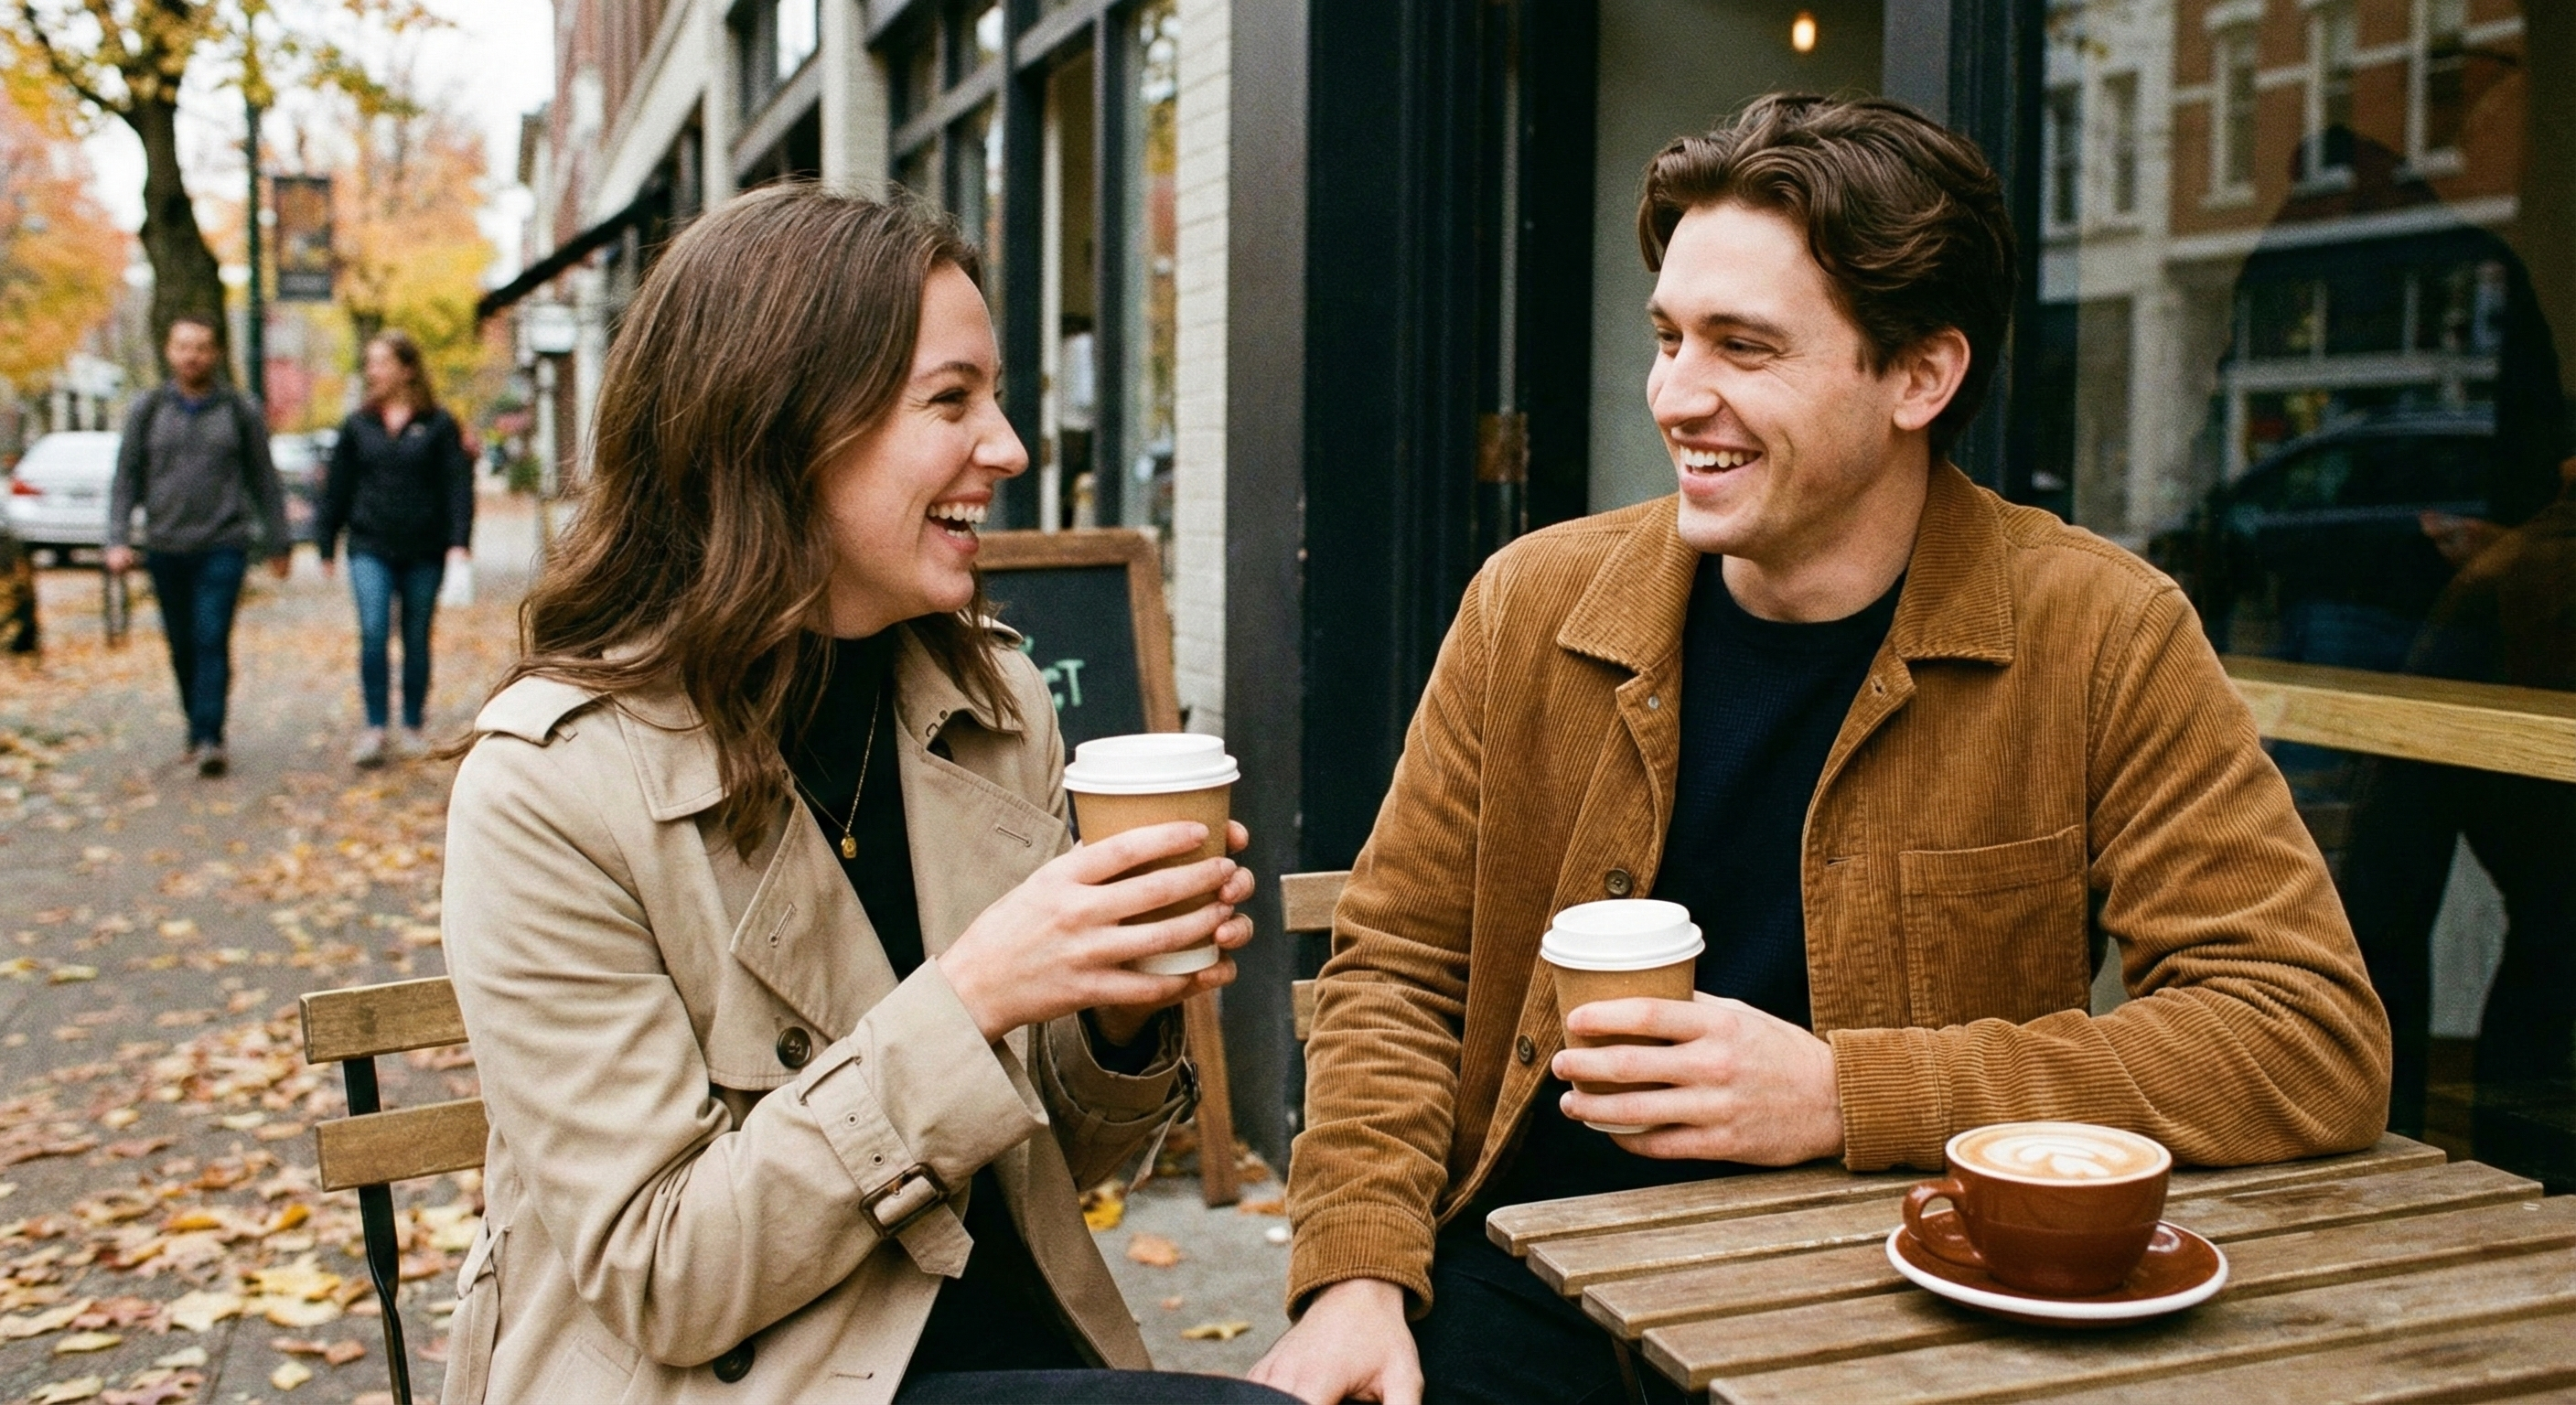
\includegraphics[width=1\linewidth]{figures/coffee.jpg}
    \end{subfigure}
    \hfill
    \begin{subfigure}[t]{0.32\linewidth}
        \includegraphics[width=1\linewidth]{figures/coffee_llava.jpg}
    \end{subfigure}
    \hfill
    \begin{subfigure}[t]{0.32\linewidth}
        \includegraphics[width=1\linewidth]{figures/coffee_sa2va.jpg}
    \end{subfigure}

    \vspace{1mm}
    \begin{minipage}{0.98\linewidth}
        \centering
        \scriptsize \textit{"Segment the cup \textbf{held by} the person in beige."}
    \end{minipage}

    \vspace{0.3cm}
    \caption{\textbf{Addressing Attention Hallucination.} 
    Unlike OMG-LLaVA~\cite{omgllava} (Center), SALMA (Right) uses structural priors to precisely ground objects with complex spatial constraints (e.g., depth, ordering), avoiding attention drift.}
    \label{fig:teaser}
\end{figure*}

However, a critical semantic-structural gap persists.
Existing MLLMs often treat visual features as abstract semantic tokens, stripping away the low-level spatial priors essential for boundary delineation.
This leads to attention hallucination: as shown in \Cref{fig:teaser}, complex spatial queries (e.g., ``\textit{the cup behind the laptop}'') cause attention to drift toward salient distractors rather than the target defined by spatial constraints.
Consequently, performance on structural benchmarks like MeVis~\cite{mevis} often lags behind human capability.

To bridge this gap, we propose SALMA, a unified framework that re-introduces structural fidelity into the attention mechanism.
We find that improving per-frame structural grounding yields substantial gains even without introducing additional temporal modules.
Unlike methods that rely on explicit user prompts (SegGPT~\cite{seggpt}) or implicit alignment (LIRA), our approach injects Mask-Biased Attention priors directly into the transformer layers.
By modulating attention weights with low-level cues from the visual backbone, we suppress noise and lock focus onto the target topology.

Our contributions are three-fold:
\begin{itemize}
    \item \textbf{Mask-Biased Attention (MBA).} We propose MBA, a novel mechanism that injects pixel-level structural priors into the MLLM's reasoning process. Uniquely, we repurpose the frozen SAM-2 decoder to generate these priors via a lightweight pre-pass, transforming the segmentation module from a passive receiver into an active spatial guide.
    \item \textbf{Dense Soft Gating.} We introduce a dense, soft gating strategy that acts as a continuous spatial constraint, avoiding the information bottleneck inherent in token-based approaches. This allows SALMA to maintain robust grounding even in complex scenarios involving heavy occlusion or motion blur.
    \item \textbf{High Efficiency and Performance.} SALMA achieves 71.9\% J\&F on Ref-DAVIS17~\cite{davis2017} (+3.4 points) and 78.4 cIoU on RefCOCOg~\cite{refcocog}, with a negligible 0.7\% latency increase. This verifies that precise structural grounding can be achieved with minimal computational overhead.
\end{itemize}

%-------------------------------------------------------------------------
\section{Related Work}
\textbf{Large Multimodal Foundation Models.}
Large Language Models (LLMs)~\cite{gpt4} have reshaped AI and motivated Multimodal LLMs (MLLMs) that align visual encoders with language backbones. Early models such as LLaVA~\cite{llava15} focus on static images, while later work scales resolution~\cite{internvl, qwen}, strengthens reasoning~\cite{llavanext}, and extends to video~\cite{videollava, videolisa}. Despite broad benchmarks~\cite{mmbench, mme, seedbench}, many MLLMs still struggle with structure because images are processed as coarse semantic tokens.

\textbf{Visual Segmentation and Grounding.}
Before unified MLLMs, referring segmentation was driven by specialist models, often with modular language--vision designs. Transformer-based methods place attention at the core of fusion; LAVT~\cite{lavt} and CRIS~\cite{cris} inject language early and use contrastive alignment. For video, ReferFormer~\cite{referformer} treats RVOS as sequence prediction. In parallel, universal segmentation advanced rapidly (e.g., SEEM~\cite{seem}, SegGPT~\cite{seggpt}), and SAM-2~\cite{sam2} introduced promptable streaming memory. These models, however, typically lack LLM-level reasoning.

\textbf{Unified Multimodal Perception.}
To connect semantic reasoning with pixel grounding, recent work integrates segmentation decoders into MLLMs~\cite{lisa, pixellm, glamm, gsva, sa2va, lira}. LISA~\cite{lisa} uses \texttt{[SEG]} tokens to invoke SAM-style decoding, PixelLM~\cite{pixellm} adopts a lightweight pixel decoder and codebook, and GLaMM~\cite{glamm}/PSALM~\cite{psalm} add region- or mask-token interfaces. Alignment-centric methods (e.g., Mask Grounding~\cite{maskgrounding}) introduce auxiliary objectives.
Notably, LIRA~\cite{lira} relies on \textit{implicit alignment}, optimizing feature discriminability through local constraints. While effective for semantics, implicit methods often struggle to resolve spatial ambiguity in complex scenes (e.g., distinguishing identical objects by position). In contrast, SALMA imposes an \textit{explicit inductive bias}: by mechanically gating attention with SAM-2's spatial prior, we force the MLLM to "look" at valid structural candidates, reducing the search space for spatial reasoning.
\section{Methodology}
\begin{figure*}[t]
    \centering
    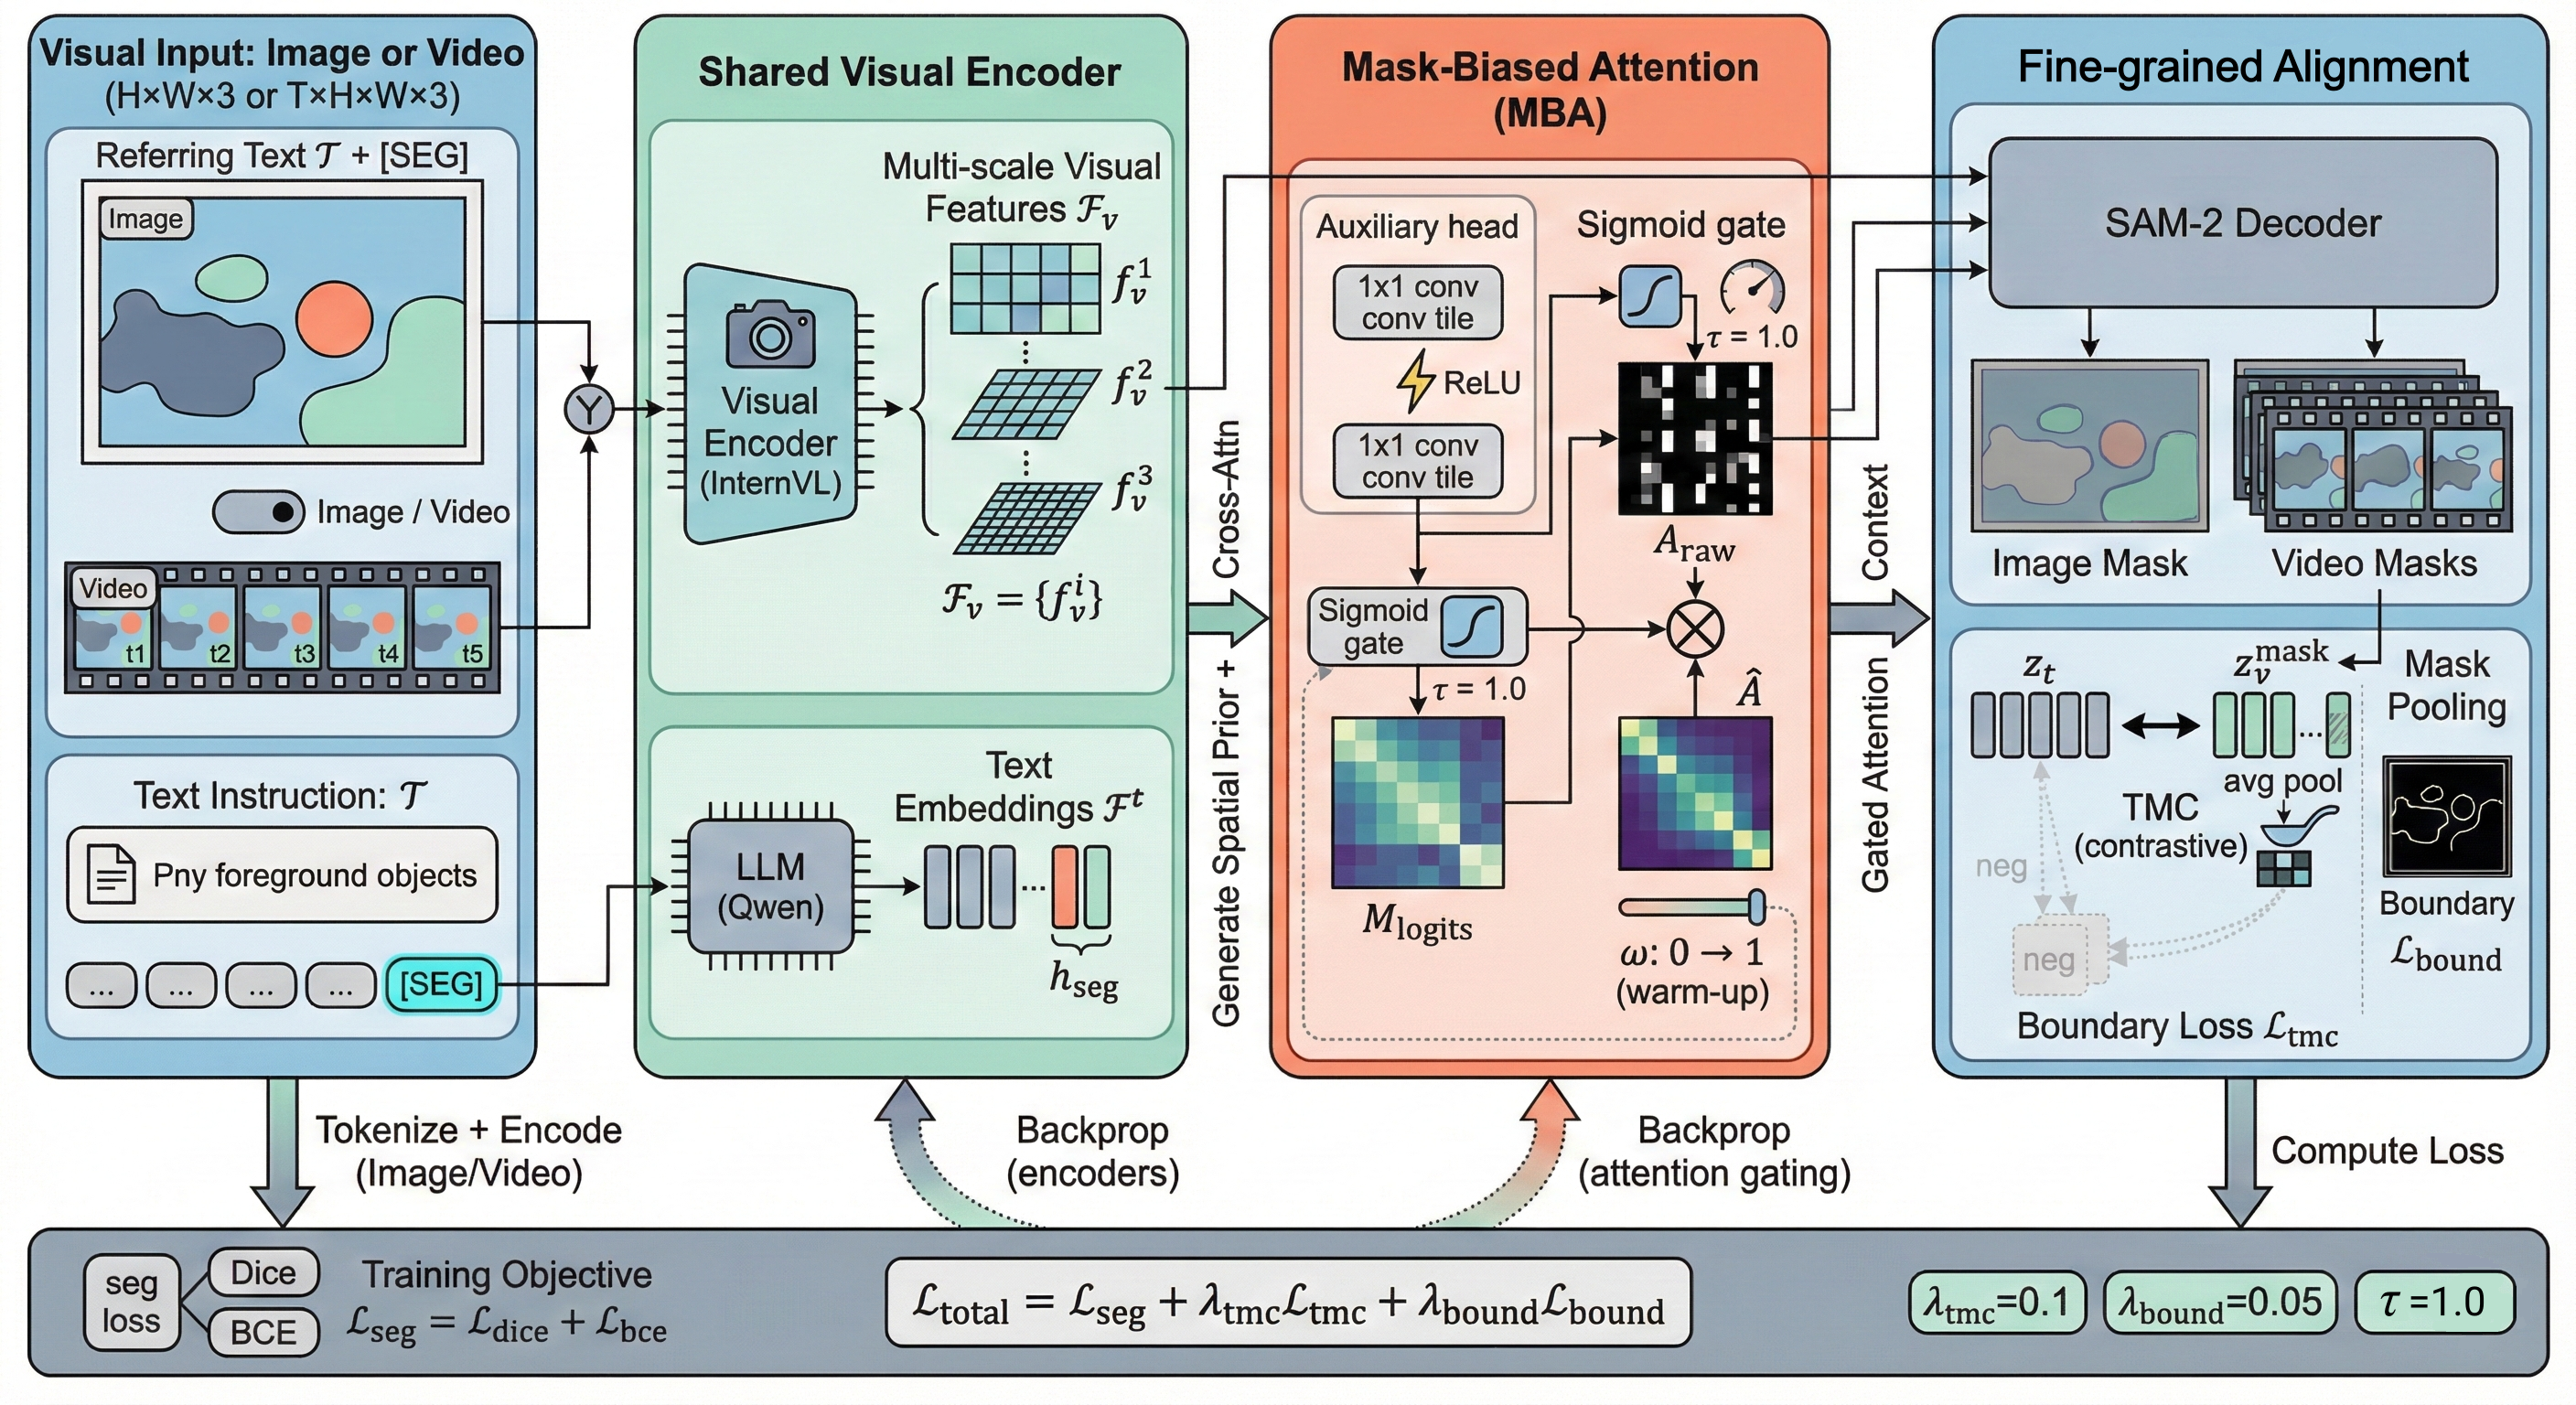
\includegraphics[width=1.0\linewidth]{figures/framework_overview.jpg}
    \caption{\textbf{Framework Overview.} \textbf{(a) Shared Visual Encoder.} Multi-scale visual features $\mathcal{F}_v$ and text embeddings are extracted.
    \textbf{(b) Mask-Biased Attention.} Instead of a separate auxiliary head, we perform a pre-pass inference using the shared SAM-2 decoder to generate a prior $\mathcal{M}_{prior}$.
    This prior is transformed via a Sigmoid into a spatial Gate $G$, which is multiplied ($\otimes$) with the Cross-Attention output features to suppress noise.
    \textbf{(c) Fine-grained Alignment.} We enforce semantic alignment via TMC Loss ($\leftrightarrow$) and structural precision via Boundary Loss (highlighted contours).}
    \label{fig:framework}
\end{figure*}
The overall pipeline of our proposed SALMA is illustrated in \Cref{fig:framework} and summarized in \Cref{alg:main}. 
The framework consists of three integrated stages: 
(1) \textbf{Shared Visual Encoder:} A visual encoder and an LLM process the input video and text to extract multi-scale visual features and text embeddings.
(2) \textbf{Mask-Biased Attention:} The proposed MBA mechanism injects pixel-level structural priors from the SAM-2 decoder into the cross-modal interaction to prevent attention drift.
(3) \textbf{Fine-grained Alignment:} Finally, the model is supervised by a dual-constraint strategy involving TMC loss and Boundary Consistency loss to ensure high-fidelity segmentation.


\subsection{Problem Formulation}
\label{sec:preliminaries}


We design SALMA as a structure-first evolution of the unified MLLM paradigm.
We adopt the \textbf{Sa2VA}~\cite{sa2va} architecture as our foundational baseline, as it efficiently integrates the semantic reasoning of MLLMs with the robust segmentation decoding of SAM-2~\cite{sam2}.
This architectural choice provides a strong starting point by combining open-ended generalization with foundational mask quality.

% [Part 2: 诊断病灶 - The Problem Hierarchy]
However, we identify a critical structural bottleneck inherent to this architecture.
While Sa2VA excels at high-level semantic recognition (e.g., identifying "a dog"), it suffers from varying degrees of degradation when handling fine-grained spatial instructions:
\begin{itemize}
    \item \textbf{Semantic Alignment:} The model effectively aligns text with visual regions for distinct objects. However, the implicit injection of the \texttt{[SEG]} token often leads to coarse localization when objects share similar semantic attributes. \textbf{This typically manifests as fragmented or incomplete masks}, where the model fails to maintain object coherence (e.g., segmenting only part of a ``pile of fries'').
    \item \textbf{Structural Hallucination:} As highlighted in Section 1, a severe limitation arises in complex reasoning scenarios (e.g., relative positioning or heavy occlusion). Since Sa2VA treats video frames as abstract 1D semantic tokens, it strips away the low-level 2D/3D spatial geometry required for precise boundary delineation. 
    Without explicit spatial constraints, the cross-modal attention mechanism exhibits attention drift, where the model \textbf{hallucinates focus on background noise or neighboring distractors} (e.g., selecting a ``large'' carrot instead of the requested ``small'' one) rather than the target's topology.
\end{itemize}
% [Part 3: 承上启下 - Motivation]
This diagnosis indicates that simply scaling data or parameters cannot resolve the structural deficit. Instead, it necessitates an explicit mechanism to re-introduce spatial priors into the MLLM's reasoning process, motivating our proposed Mask-Biased Attention within the SALMA framework.

\subsection{Mask-Biased Attention}
\label{sec:mba}

Standard cross-attention often introduces noise by allowing global interaction. We propose Mask-Biased Attention (MBA) to strictly gate semantic injection using low-level spatial priors.

\textbf{Spatial Prior via Auxiliary Execution.}
To obtain structural guidance without training a separate head, we leverage the \textit{shared} SAM-2 decoder for a lightweight pre-pass. Algorithmically, we supply a constant dummy negative point (label -1) at $(0,0)$ during both training and inference. This fixed prompt satisfies the decoder's interface while allowing the mask generation to be primarily driven by SAM-2's learned internal saliency prior, effectively independent of specific user guidance.
During pre-pass, output logits are detached from the computation graph; during final decoding, decoder weights are fine-tuned end-to-end.
This dual-mode usage extracts robust priors without memory overhead. For video inputs, priors are generated independently per frame to prevent error accumulation, while SAM-2's internal memory maintains temporal consistency during the final decoding stage.

\textbf{Visual-Query Attention with Top-K Routing.}
We invert the standard interaction direction by treating visual features $\mathcal{F}_v \in \mathbb{R}^{HW \times C}$ as Queries and text tokens $\mathcal{F}_t$ as Keys/Values. To prevent attention from being diluted by functional words (e.g., articles, prepositions), we employ a Top-K Token Routing strategy that acts as a \textit{semantic denoiser}. 
We first compute a scalar importance score $s_i$ for each token via an MLP router, and then select the top-$K$ subset $\hat{\mathcal{F}}_t$ for attention. We set $K=2$ by default. This heuristic is grounded in the linguistic observation that referring expressions predominantly pivot on a core Subject-Attribute pair (e.g., ``\textit{small carrot}'' $\to$ [carrot, small] or ``\textit{man in red}'' $\to$ [man, red]). While longer sentences exist, the discriminative information is typically concentrated in 1-2 keywords. Empirical tests suggested that dynamic $K$ introduced unnecessary latency and routing noise, whereas a fixed $K=2$ acts as an effective semantic bottleneck, forcing the model to identify the most critical cues:
\begin{equation}
    s_i = \text{MLP}(t_i), \quad \hat{\mathcal{F}}_t = \{t_i \mid i \in \text{TopK}(s, K)\}
\end{equation}
The retrieved semantic features $\mathcal{O}_{attn}$ are then computed via standard Multi-Head Attention (MHA) between the visual queries and the filtered text tokens.
\begin{figure}[t]
    \centering
    \includegraphics[width=1.0\linewidth]{figures/mechanism.jpg}
    \caption{\textbf{The Mask-Biased Attention (MBA) Mechanism.} 
    We visualize the transformation from the noisy global attention $A_{\text{raw}}$ to the refined structure-aware output $\hat{A}$. 
    The \textbf{Mask Prior ($G$)}, acting as a soft spatial filter, is element-wise multiplied ($\otimes$) with the raw features. 
    This process effectively \textbf{suppresses background hallucinations} and confines semantic reasoning strictly within the target's topology.}
    \label{fig:mba_module}
\end{figure}

\textbf{Mask-Gated Modulation.}
Different from implicit bias mechanisms, we explicitly modulate the attention output features using the generated spatial prior, as illustrated in Figure \ref{fig:mba_module}.
We apply this gating to the cross-attention output rather than the internal probability map. This modulates semantic flow without distorting the probabilistic alignment between tokens.

We first normalize the logits $\mathcal{M}_{logits}$ into a soft spatial gate $G$ using a temperature-scaled Sigmoid. The structure-aware features are then injected into the visual backbone via a gated residual connection:
\begin{equation}
    G = \sigma\left(\frac{\mathcal{M}_{logits}}{\tau_{gate}}\right), \quad \mathcal{F}_{v}' = \mathcal{F}_v + \gamma \cdot (\mathcal{O}_{attn} \odot G)
\end{equation}
where $G$ is resized via bilinear interpolation to match the spatial resolution $H \times W$ of the visual query features $\mathcal{F}_v$. $\mathcal{O}_{attn}$ is the projected output of the Multi-Head Attention, $\odot$ denotes element-wise multiplication, and $\gamma$ is a learnable scaling factor.
This learnable $\gamma$ is crucial for robustness: it effectively acts as a confidence gate. If the pre-pass mask is noisy or incorrect (e.g., in low-contrast camouflage), the model can learn to suppress $\gamma$ via the task loss, falling back to standard attention. This prevents the "bad prior" from catastrophically misleading the segmentation.

\textbf{Soft Constraint vs. Hard Tokens.}
A critical distinction of our approach is the nature of the spatial injection. Existing methods like LISA~\cite{lisa} or GLaMM~\cite{glamm} rely on ``hard'' tokens (e.g., \texttt{[SEG]}) to trigger segmentation. This creates a representational bottleneck: the complex spatial intent must be compressed into a single vector, often leading to ``all-or-nothing'' failures if the token embedding is misaligned.
In contrast, MBA imposes a \textit{soft, dense constraint} over the entire visual feature map. The residual connection $\mathcal{F}_{v}' = \mathcal{F}_v + \dots$ ensures that the original semantic information is never discarded, only refined. If the prior is incorrect, the learnable $\gamma$ can converge to zero, allowing the model to revert to standard attention, a robustness property structurally impossible in hard-token architectures. Moreover, token condensation inevitably discards high-frequency spatial details. By maintaining the full resolution of the visual feature map, our dense gating preserves the fine-grained geometric cues necessary for segmenting small or thin objects, which are prone to vanishing in token-based bottlenecks.

\subsection{Fine-grained Alignment}
\label{sec:alignment}

% [新增] Motivation 段落 - 解释为什么要加 TMC 和 Boundary Loss
MBA injects spatial priors, but precise masks still benefit from explicit fine-grained supervision. Without targeted constraints, features can drift to semantically similar yet spatially distinct instances (e.g., adjacent "red cars"). We therefore apply a dual-constraint strategy (TMC + boundary), as shown in the \textbf{Right} panel of \Cref{fig:framework}.

\textbf{Text-Mask Contrastive Learning.}
To prevent the visual features from drifting away from the textual instructions during the decoding process, we enforce a semantic consistency constraint.
Specifically, we extract the region-level visual feature $z_v^{mask}$ by average-pooling the feature map $\mathcal{F}_v$ over the ground-truth foreground region $\mathcal{M}^{gt}$. We use the ground-truth mask during training to ensure stable semantic alignment, decoupling it from early-stage segmentation errors.
Let $z_t$ be the embedding of the special \texttt{[SEG]} token corresponding to the referring expression. We employ a Symmetric InfoNCE loss where \textbf{negatives are constructed from other text-image pairs within the same batch}, maximizing the mutual information between the matched text-visual pair $(z_t, z_v^{mask})$:
\begin{equation}
    \mathcal{L}_{tmc} = \mathcal{L}_{v \to t} + \mathcal{L}_{t \to v}
\end{equation}
where both directions (vision-to-text and text-to-vision) are normalized by temperature $\tau_{tmc}$.
This symmetric objective explicitly aligns the latent space of the "attended region" with the language instruction, ensuring the model not only looks at the right place but also understands the correct semantics.
%-------------------------------------------------------------------------
\begin{algorithm}[t]
    \caption{Overall Training Pipeline}
    \label{alg:main}
    \begin{algorithmic}[1]
        \STATE \textbf{Input:} Image $I$, Language Instruction $T$
        \STATE \textbf{Output:} Segmentation Mask $\mathcal{M}$
        \STATE \textbf{Parameters:} Gate Temp $\tau_{gate}=1.0$, Routing $K=2$, loss weights $\lambda_{tmc}, \lambda_{bound}$
        
        \vspace{0.5em}
        \STATE \textbf{Stage 1: Multimodal Feature Extraction}
        \STATE $F_v \gets \text{VisualBackbone}(I)$ \hfill $\triangleright$ \textit{Extract multi-scale visual features}
        \STATE $F_t \gets \text{LLM}(T)$ \hfill $\triangleright$ \textit{Extract text embeddings}
        
        \vspace{0.5em}
        \STATE \textbf{Stage 2: Structural Prior Generation (Pre-pass)}
        \STATE $P_{bg} \gets \{(0, 0), \text{label}=-1\}$ \hfill $\triangleright$ \textit{Background point prompt}
        \STATE \textbf{Freeze} SAM-2 Decoder parameters \hfill $\triangleright$ \textit{Stop gradient flow}
        \STATE $\mathcal{M}_{logits} \gets \text{SAM2Decoder}(F_v, P_{bg})$ 
        \STATE $G \gets \sigma(\mathcal{M}_{logits} / \tau_{gate})$ \hfill $\triangleright$ \textit{Generate soft spatial gate}
        \STATE \textbf{Unfreeze} SAM-2 Decoder
        
        \vspace{0.5em}
        \STATE \textbf{Stage 3: Mask-Biased Attention (MBA)}
        \FOR{each layer $l$ in VLM}
            \STATE $S \gets \text{MLP}(F_t)$ \hfill $\triangleright$ \textit{Predict token saliency}
            \STATE $\hat{F}_t \gets \text{TopK}(F_t, S, K)$ \hfill $\triangleright$ \textit{Select top-K relevant tokens}
            \STATE $O_{attn} \gets \text{CrossAttn}(Q=F_v, K=\hat{F}_t, V=\hat{F}_t)$
            \STATE \textcolor{gray}{\# Gated Injection: Semantic $\times$ Structural Prior}
            \STATE $F_v \gets F_v + \gamma_l \cdot (O_{attn} \odot G)$ 
        \ENDFOR
        
        \vspace{0.5em}
        \STATE \textbf{Stage 4: Final Decoding \& Optimization}
        \STATE $\hat{\mathcal{M}} \gets \text{SAM2Decoder}(F_v, T)$ \hfill $\triangleright$ \textit{Text-conditioned decoding}
        
        \STATE $\mathcal{L}_{seg} \gets \mathcal{L}_{dice}(\hat{\mathcal{M}}, \mathcal{M}^{gt}) + \mathcal{L}_{bce}(\hat{\mathcal{M}}, \mathcal{M}^{gt})$
        \STATE $z_v^{mask} \gets \text{Pool}(F_v, \mathcal{M}^{gt})$ \hfill $\triangleright$ \textit{Target region features}
        \STATE $\mathcal{L}_{tmc} \gets \text{Contrastive}(z_v^{mask}, F_t)$ \hfill $\triangleright$ \textit{Semantic Alignment}
        \STATE $\mathcal{L}_{bound} \gets \text{BoundaryLoss}(\hat{\mathcal{M}}, \mathcal{M}^{gt})$ \hfill $\triangleright$ \textit{Structural Precision}
        \STATE $\mathcal{L}_{total} \gets \mathcal{L}_{seg} + \lambda_{tmc} \mathcal{L}_{tmc} + \lambda_{bound} \mathcal{L}_{bound}$
        
        \STATE \textbf{Update} model parameters using $\nabla \mathcal{L}_{total}$
    \end{algorithmic}
\end{algorithm}

%-------------------------------------------------------------------------
\textbf{Boundary Consistency Constraint.}
Standard binary cross-entropy (BCE) and Dice losses primarily focus on the overall mask area but are insensitive to boundary errors.
In video segmentation, however, fuzzy boundaries are a major source of qualitative degradation (e.g., temporal jitter).
We incorporate a Boundary Loss $\mathcal{L}_{bound}$ that measures the discrepancy between predicted and ground-truth edge maps:
\begin{equation}
    \mathcal{L}_{bound} = \|\nabla \hat{\mathcal{M}} - \nabla \mathcal{M}^{gt}\|_1
\end{equation}
where $\nabla \hat{\mathcal{M}}$ and $\nabla \mathcal{M}^{gt}$ denote the gradient magnitudes of the predicted and ground-truth masks, respectively, computed via Sobel edge detection with $3{\times}3$ kernels.
We use the standard $3{\times}3$ kernel size following common practice in boundary-aware losses; larger kernels (e.g., $5{\times}5$) were tested but showed no significant improvement while increasing computational cost.
By optimizing this boundary-specific objective, the model is explicitly penalized for edge inaccuracies, acting as a fine-grained sharpener for the output masks.


\subsection{Unified Training Objective}
We formulate a unified optimization target that balances global semantic fidelity with local structural precision:

% [原有公式部分]
Our total loss function is defined as:
\begin{equation}
    \mathcal{L}_{total} = \mathcal{L}_{seg} + \lambda_{tmc}\,\mathcal{L}_{tmc} + \lambda_{bound}\,\mathcal{L}_{bound}
\end{equation}

where:
\begin{itemize}
    \item $\mathcal{L}_{seg} = \mathcal{L}_{dice} + \mathcal{L}_{bce}$: This is the standard linear combination of Dice loss and Binary Cross-Entropy loss used in SAM-2, responsible for the general mask quality.
    \item $\mathcal{L}_{tmc}$: The Text-Mask Contrastive loss enforces semantic fidelity.
    \item $\mathcal{L}_{bound}$: The Boundary loss enforces high-frequency structural precision.
\end{itemize}
\begin{table*}[t]
    \centering
    \caption{\textbf{Comparison with State-of-the-Art Methods.} We report cIoU for image referring segmentation tasks, $\mathcal{J}\&\mathcal{F}$ for video segmentation tasks, and standard metrics for multimodal understanding.
    The best results are highlighted in \textbf{bold}. SALMA achieves leading performance among unified MLLMs on video segmentation tasks and complex referring scenarios (e.g., RefCOCOg), while maintaining competitive general understanding capabilities.}
    \label{tab:sota_comparison}
    \renewcommand{\arraystretch}{1.1}
    \resizebox{\textwidth}{!}{
    \begin{tabular}{l|ccc|ccc|cc|ccc|ccc}
        \toprule
        \multirow{3}{*}{\textbf{Method}} & \multicolumn{8}{c|}{\textbf{Image Segmentation}} & \multicolumn{3}{c|}{\textbf{Video Segmentation}} & \multicolumn{3}{c}{\textbf{Image Chat}} \\
         & \multicolumn{3}{c|}{RefCOCO~\cite{refcoco}} & \multicolumn{3}{c|}{RefCOCO+~\cite{refcoco}} & \multicolumn{2}{c|}{RefCOCOg~\cite{refcocog}} & \multirow{2}{*}{Ref-DAVIS17~\cite{davis2017}} & \multirow{2}{*}{Ref-YouTube-VOS~\cite{ytvos}} & \multirow{2}{*}{MeVis~\cite{mevis}} & \multirow{2}{*}{MME~\cite{mme}} & \multirow{2}{*}{MMB~\cite{mmbench}} & \multirow{2}{*}{SEED~\cite{seedbench}} \\
      
        & Val & TestA & TestB & Val & TestA & TestB & Val & Test & & & & & & \\
        \midrule
        LLAVA-1.5-13B~\cite{llava15} & - & - & - & - & - & - & - & - & - & - & - & 1531(+) & 68.8 & 70.1 \\
        Video-LLaVA-7B~\cite{videollava} & - & - & - & - & - & - & - & - & - & - & - & - & 60.9 & - \\
        LLaMA-VID-7B~\cite{llamavid} & - & - & - & - & - & - & - & - & - & - & - & 1521(+) & 65.1 & 59.9 \\
        mPLUG-Owl3-8B~\cite{mplugowl3} & - & - & - & - & - & - & - & - & - & - & - & - & 77.6 & - \\
        InternVL2-8B~\cite{internvl} & - & - & - & - & - & - & - & - & - & - & - & - & 81.7 & 76.2 \\
        PixelLM-7B~\cite{pixellm} & 73.0 & - & - & 66.3 & - & - & 69.3 & - & - & - & - & 309/135 & 17.4 & - \\
        PixelLM-13B~\cite{pixellm} & 73.0 & 76.5 & 68.2 & 66.3 & 71.7 & 58.3 & 69.3 & 70.5 & - & - & - & 309/135 & 17.4 & - \\
        LaSagnA~\cite{lasagna} & 76.8 & - & - & 66.4 & - & - & 70.6 & - & - & - & - & 0/0 & 0.0 & - \\
        LISA-7B~\cite{lisa} & 74.1 & 76.5 & 71.1 & 62.4 & 67.4 & 56.5 & 66.4 & 68.5 & - & - & - & 1/1 & 0.4 & - \\
        LISA-GLEE~\cite{lisaglee} & 76.4 & 78.2 & 73.8 & 67.3 & 71.3 & 62.3 & 71.6 & 72.4 & - & - & - & - & - & - \\
        GLaMM~\cite{glamm} & 79.5 & 83.2 & 76.9 & 72.6 & 78.7 & 64.6 & 74.2 & 74.9 & - & - & - & 14/9 & 36.8 & - \\
        LLaVA-G-7B~\cite{llavag} & 77.1 & - & - & 68.8 & - & - & 71.5 & - & - & - & - & - & - & - \\
        GSVA~\cite{gsva} & 77.2 & 78.9 & 73.5 & 65.9 & 69.6 & 59.8 & 72.7 & 73.3 & - & - & - & - & - & - \\
        OMG-LLaVA-8B~\cite{omgllava} & 75.6 & 77.7 & 71.2 & 65.6 & 69.7 & 58.9 & 70.7 & 70.2 & - & - & - & 1177/235 & 47.9 & 56.5 \\
        PSALM~\cite{psalm} & \textbf{83.6} & \textbf{84.7} & \textbf{81.6} & 72.9 & 75.5 & 70.1 & 73.8 & 74.4 & - & - & - & - & 52.5 & - \\
        VideoLISA-3.8B~\cite{videolisa} & 73.8 & - & - & 63.4 & - & - & 68.3 & - & 68.8 & 63.7 & 44.4 & - & - & - \\
        VISA-13B~\cite{visa} & 72.4 & - & - & 59.8 & - & - & 65.5 & - & 70.4 & 63.0 & 44.5 & - & - & - \\
        \midrule
        Sa2VA-1B (Base)* & 79.6 & 82.7 & 76.5 & 73.6 & 79.0 & 66.6 & 77.8 & 77.5 & 68.5 & 65.3 & 41.7 & \textbf{1487/433} & \textbf{71.9} & \textbf{71.0} \\
        \textbf{SALMA} & 80.4 & 83.2 & 77.7 & \textbf{74.8} & \textbf{80.0} & \textbf{68.9} & \textbf{78.0} & \textbf{78.4} & \textbf{71.9} & \textbf{67.0} & \textbf{46.0} & 1421/353 & 71.2 & 69.9 \\
        \bottomrule
    \end{tabular}}
\end{table*}

\textbf{Hyper-parameter Selection.}
We set $\lambda_{tmc}=0.1$ and $\lambda_{bound}=0.05$ to balance semantic alignment and structural precision.
For the gating temperature, we set $\tau_{gate}=1.0$, which corresponds to applying the standard Sigmoid function without any scaling.
This choice directly uses the SAM-2 decoder's output logits as the spatial prior, preserving the decoder's learned confidence distribution.


\section{Experiments}

\subsection{Implementation Details}
\textbf{Architecture.} We build on Sa2VA-1B, using InternVL2.5-1B~\cite{internvl25new} (with InternViT encoder) as the MLLM backbone and SAM-2's Hiera-L as the segmentation image encoder. The SAM-2 mask decoder serves dual roles: frozen for prior extraction during pre-pass, fine-tuned for final text-conditioned decoding.

\textbf{Training.} We train end-to-end for 1 epoch on 4$\times$ RTX 5090 GPUs using AdamW ($\beta_1{=}0.9$, $\beta_2{=}0.999$, weight decay 0.05), learning rate $4{\times}10^{-5}$ with cosine decay, DeepSpeed, and BF16 precision.
Our dataset mixes image referring segmentation (RefCOCO/+/g~\cite{refcoco,refcocog} 4$\times$, GCG), video segmentation (MeVis 4$\times$, ReVOS~\cite{visa} 10$\times$, Ref-YouTube-VOS/Ref-DAVIS~\cite{ytvos,davis2017} 4$\times$, SAM-2 SA-V 4$\times$), and general instructions (LLaVA-1.5~\cite{llava15}, Video-ChatUniVi~\cite{chatunivi24}, Osprey-724k~\cite{osprey24}). We use official train splits for all video benchmarks.

\textbf{Hyper-parameters.} We set $\lambda_{tmc}{=}0.1$, $\lambda_{bound}{=}0.05$, and $\tau_{gate}{=}1.0$. A 5\% linear warm-up is applied to auxiliary loss weights and $\gamma$ to prevent disrupting pre-trained features.

\subsection{Evaluation Benchmarks}
To rigorously verify SALMA's structure-aware capabilities, we conduct comprehensive evaluations across three complementary domains:

\textbf{Referring Image Segmentation.} We evaluate on the classic RefCOCO, RefCOCO+, and RefCOCOg benchmarks. These datasets test the model's ability to ground static objects from natural language descriptions. RefCOCOg is particularly challenging due to its longer, more complex expressions. We report performance using the standard Cumulative Intersection-over-Union metric.

\textbf{Referring Video Segmentation.} To assess structural stability in dynamic scenes, we test on Ref-DAVIS17 and Ref-YouTube-VOS. These benchmarks require the model to maintain consistent tracking of a referred object across video frames. We report the $\mathcal{J}\&\mathcal{F}$ mean score, which aggregates region similarity ($\mathcal{J}$) and boundary contour accuracy ($\mathcal{F}$).

\textbf{Motion-Centric Understanding.} We utilize the MeVis benchmark, which features queries explicitly dependent on motion cues (e.g., ``the fish swimming to the left''). This tests whether our structural priors remain robust under complex temporal dynamics.

\subsection{Comparison with Leading MLLMs}
We present a comprehensive comparison of our method (SALMA) against leading Multi-Modal Large Language Models (MLLMs).
As shown in \Cref{tab:sota_comparison}, we evaluate performance across three distinct dimensions: image referring segmentation, video segmentation, and general multi-modal understanding.

\textbf{Quantitative Analysis.} As shown in \Cref{tab:sota_comparison}, our method outperforms baselines across segmentation tasks. On RefCOCOg, we achieve 78.4 cIoU, supporting the effectiveness of our structure-aware attention and alignment objectives. For video, we achieve 71.9 J\&F on Ref-DAVIS17 (+3.4 over baseline) and 67.0 J\&F on Ref-YouTube-VOS (+1.7 over baseline), validating our structural priors on standard benchmarks.

\textbf{Generalization-Specialization Trade-off.} We observe modest decreases on general MLLM benchmarks.
However, our core task improvements (+3.4 on Ref-DAVIS17, +1.7 on Ref-YouTube-VOS) substantially outweigh this degradation.
Notably, PSALM~\cite{psalm} reports 52.5 on MMBench, while our model achieves 71.2, suggesting our implicit gating better retains general reasoning capability than explicit token-based approaches.
We argue that this is a justifiable \textbf{Specialization for Fine-grained Grounding}: in practical agentic applications, precise physical localization is often more critical than generic QA capabilities, making this trade-off highly favorable for grounding-centric tasks.

\subsection{Ablation Study}
We investigate the separate contributions of each component in \Cref{tab:ablation_component}. The vanilla Sa2VA baseline exhibits substantial attention drift due to global cross-modal interaction without spatial constraints. Introducing MBA alone yields the largest single improvement (+1.31 J\&F on DAVIS, +0.76 cIoU on RefCOCOg), demonstrating that structural gating effectively suppresses attention hallucination. Incorporating TMC and Boundary losses further refines semantic alignment and edge precision, with the full model achieving optimal performance (71.87 J\&F / 78.42 cIoU), validating our dual-constraint strategy.

\begin{table}[t]
    \centering
    \caption{\textbf{Ablation Study of Components.} We progressively add Mask-Biased Attention, Text-Mask Contrastive and Boundary Loss.}
    \label{tab:ablation_component}
    \small
    \begin{tabular}{l|cc}
        \toprule
        Configuration & DAVIS (J\&F) & RefCOCOg (test) \\
        \midrule
        Baseline (Sa2VA) & 68.52 & 77.45 \\
        + MBA & 69.83 & 78.21 \\
        + MBA + TMC & 71.04 & 78.28 \\
        + MBA + TMC + Bound & \textbf{71.87} & \textbf{78.42} \\
        \bottomrule
    \end{tabular}
\end{table}

\begin{table}[t]
    \centering
    \caption{\textbf{Analysis of Feature Modulation.} Comparing our simplified spatial gating vs. complex FiLM modulation.
    \textcolor{red}{Red text} indicates a performance drop relative to our full model.}
    \label{tab:ablation_film}
    \small
    \begin{tabular}{l|cc}
        \toprule
        Method & Ref-DAVIS17 & MeVis ($\text{Val}_{u}$) \\
        \midrule
        Ours (Full) & \textbf{71.87} & \textbf{53.37} \\
        Ours (w/ FiLM) & 68.13 \textcolor{red}{(-3.74)} & 47.46 \textcolor{red}{(-5.91)} \\
        \bottomrule
    \end{tabular}
\end{table}

\textbf{Impact of Residual FiLM.}
We investigated a more complex modulation mechanism called Residual FiLM, where feature-wise affine transformations are applied in addition to our spatial gating.
As shown in \Cref{tab:ablation_film}, FiLM significantly degrades performance (DAVIS -3.74, MeVis -5.91). We attribute this to FiLM’s over-aggressive feature modulation distorting the pre-trained statistical properties.
Unlike our lightweight gating mechanism that preserves the original feature distribution while selectively injecting structural priors, FiLM applies a full affine transformation ($\gamma \cdot \mathcal{F} + \beta$) that fundamentally distorts the learned visual representations.
This distortion is particularly harmful because: (1) the SAM-2 decoder was pre-trained on features with specific statistical properties, and aggressive modulation breaks this assumption; (2) the semantic richness encoded in the MLLM features is corrupted, impairing both structural (DAVIS) and motion-centric (MeVis) reasoning.

This finding validates our design choice of minimal intervention: the gating mechanism should enhance attention focus without distorting the underlying feature space.


\textbf{Quantitative Saliency Bias Analysis.}
To rigorously evaluate the impact of our class-agnostic priors on small, non-salient targets, we conducted a stratified evaluation on the RefCOCOg validation set, partitioning objects by their area ratio ($<1\%$, $<2\%$, $<5\%$).
As shown in \Cref{tab:ablation_saliency}, our method consistently outperforms the baseline on objects occupying $<2\%$ area (+1.2 cIoU) and $<5\%$ area (+2.2 cIoU), directly addressing the concern that mask priors might suppress non-salient objects.
We observe a performance drop only on extreme outliers ($<1\%$ area), where our method trails the baseline (-3.9 cIoU). However, it is crucial to maximize the broader context: this subset represents merely \textbf{0.7\%} of the entire dataset ($N=35$). For the vast majority (\textbf{99.3\%}) of cases, including other small objects, SALMA provides superior grounding. This indicates a highly favorable trade-off: we accept a minor degradation in extremely rare, sub-pixel scenarios to gain significant robustness in realistic, complex spatial queries.

\begin{table}[t]
    \centering
    \caption{\textbf{Saliency Bias Analysis on RefCOCOg (Val).} We report cIoU scores partitioned by object area ratio ($<1\%, <2\%, <5\%$), where $N$ denotes the number of samples in each subset. Our method demonstrates robust improvements on small objects ($<2\%$ and $<5\%$), effectively countering saliency bias concerns.}
    \label{tab:ablation_saliency}
    \small
    \begin{tabular}{l|ccc|c}
        \toprule
        Method & $<1\%$ ($N=35$) & $<2\%$ ($N=151$) & $<5\%$ ($N=1559$) & All ($N=4896$) \\
        \midrule
        Baseline (Sa2VA) & \textbf{37.1} & 47.7 & 68.0 & 77.8 \\
        \textbf{Ours} & 33.2 & \textbf{48.9} & \textbf{70.2} & \textbf{78.0} \\
        \bottomrule
    \end{tabular}
\end{table}


\begin{table}[t]
    \centering
    \caption{\textbf{Computational Cost Analysis on 1024$\times$1024 resolution.} We report parameters and FLOPs for major components. The SALMA pre-pass (Gating + Decoder) introduces negligible overhead ($\sim$0.04\%) relative to the backbone encoders.}
    \label{tab:flops}
    \small
    \begin{tabular}{l|cc}
        \toprule
        Component & Params (M) & FLOPs (G) \\
        \midrule
        Vision Encoder (InternViT) & 304.0 & 1614.1 \\
        SAM-2 Image Encoder (Hiera) & 212.7 & 810.5 \\
        Visual Projector & 4.5 & 1.2 \\
        \textbf{SALMA Pre-Pass (Gating + Decoder)} & 12.0 & $<$1.0 \\
        \bottomrule
    \end{tabular}
\end{table}

\textbf{Inference Efficiency.}
A potential concern with multi-stage inference approaches is the computational cost.
To evaluate this, we benchmarked the inference speed on a standard NVIDIA RTX 5090 GPU environment using the DAVIS validation set (batch size=1).
Our method achieves 17.84 FPS, exhibiting a negligible latency increase compared to the Sa2VA-1B baseline (17.97 FPS).
This minimal drop ($\sim$0.7\%) is consistent with the computational accounting in \Cref{tab:flops} (Table~5): the SALMA-specific pre-pass (Gating + SAM-2 decoder) introduces $<1$ GFLOP at 1024$\times$1024 resolution and only $\sim$12M parameters, which is negligible relative to the heavy vision encoders (InternViT + SAM-2 Hiera) that dominate the overall budget.
Furthermore, because the pre-pass operates on detached features and does not store gradients, the additional memory footprint remains minimal, validating our design for practical real-time applications.

\subsection{Visualization}

To intuitively understand the effectiveness of our Structure-Aware framework, we provide qualitative comparisons and attention visualizations.
\begin{figure*}[t!]
    \centering
    % Define widths
    \setlength{\tabcolsep}{1pt}
    \renewcommand{\arraystretch}{0.5}

    % Headers
    \begin{minipage}{0.31\linewidth}
        \centering \small \textbf{Input / Instruction}
    \end{minipage}
    \hfill
    \begin{minipage}{0.31\linewidth}
        \centering \small \textbf{Baseline (Sa2VA-1B)}
    \end{minipage}
    \hfill
    \begin{minipage}{0.31\linewidth}
        \centering \small \textbf{Ours (Structure-Aware)}
    \end{minipage}

    \vspace{1mm}

    % --- Row 1: Carrot ---
    \begin{subfigure}[b]{0.31\linewidth}
        \includegraphics[width=\linewidth]{figures/11298_orig.jpg}
    \end{subfigure}%
    \hfill
    \begin{subfigure}[b]{0.31\linewidth}
        \includegraphics[width=\linewidth]{figures/11298_baseline_viz(2).jpg}
    \end{subfigure}%
    \hfill
    \begin{subfigure}[b]{0.31\linewidth}
        \includegraphics[width=\linewidth]{figures/11298_ours_viz.jpg}
    \end{subfigure}

    \vspace{0.5mm}
    \begin{minipage}{0.98\linewidth}
        \centering
        \small \textit{``Segment a small carrot that has a larger carrot to its left and onions to its right.''}
    \end{minipage}

    \vspace{2mm}

    % --- Row 2: Fries ---
    \begin{subfigure}[b]{0.31\linewidth}
        \includegraphics[width=\linewidth]{figures/22463_orig.jpg}
    \end{subfigure}%
    \hfill
    \begin{subfigure}[b]{0.31\linewidth}
        \includegraphics[width=\linewidth]{figures/22463_baseline_viz(2).jpg}
    \end{subfigure}%
    \hfill
    \begin{subfigure}[b]{0.31\linewidth}
        \includegraphics[width=\linewidth]{figures/22463_ours_viz.jpg}
    \end{subfigure}

    \vspace{0.5mm}
    \begin{minipage}{0.98\linewidth}
        \centering
        \small \textit{``Segment the fry on top of the pile of fries.''}
    \end{minipage}

    \caption{\textbf{Qualitative Comparison on Complex Referring Expressions.} 
    \textbf{Top Row:} Our model successfully handles complex spatial relationships (e.g., ``small'', ``to its left''), whereas the baseline incorrectly segments the distracting neighbor.
    \textbf{Bottom Row:} In highly cluttered scenes (pile of fries), our method produces masks with superior boundary crispness and completeness compared to the fragmented outputs of the baseline.}
    \label{fig:viz_comparison}
\end{figure*}

\textbf{Qualitative Results.}
As shown in \Cref{fig:viz_comparison}, in the first row, the instruction ``\textit{a small carrot...to its left}'' requires spatial reasoning; the baseline segments the wrong object, illustrating the \textbf{Structural Hallucination} problem defined in \Cref{sec:preliminaries}. Our model, guided by MBA gating, successfully suppresses the distractor.
In the second row, the baseline output is fragmented, suffering from the \textbf{Semantic Alignment} deficit. In contrast, our method produces coherent masks with sharp boundaries, validating the effectiveness of our fine-grained alignment objectives.
\begin{figure}[t!]
    \centering
    \setlength{\tabcolsep}{1pt} 
    
    % Row 1: Carrot (11298)
    \begin{subfigure}[b]{0.32\linewidth}
        \includegraphics[width=\linewidth]{figures/11298_orig.jpg}
        % \caption{Input}
    \end{subfigure}
    \hfill
    \begin{subfigure}[b]{0.32\linewidth}
        \includegraphics[width=\linewidth]{figures/11298_baseline_attncircle.png}
        % \caption{Baseline}
    \end{subfigure}
    \hfill
    \begin{subfigure}[b]{0.32\linewidth}
        \includegraphics[width=\linewidth]{figures/11298_ours_attn.jpg}
        % \caption{Ours}
    \end{subfigure}

    \vspace{1mm}

    % Row 2: Fries (22463)
    \begin{subfigure}[b]{0.32\linewidth}
        \includegraphics[width=\linewidth]{figures/22463_input.jpg}
        \caption{Input}
    \end{subfigure}
    \hfill
    \begin{subfigure}[b]{0.32\linewidth}
        \includegraphics[width=\linewidth]{figures/22463_baseline_attncircle.png}
        \caption{Baseline}
    \end{subfigure}
    \hfill
    \begin{subfigure}[b]{0.32\linewidth}
        \includegraphics[width=\linewidth]{figures/22463_ours_attn.jpg}
        \caption{Ours}
    \end{subfigure}
    \vspace{-2mm}
    \caption{\textbf{Visualization of the structure-aware ``Spotlight Effect.''} We compare the MLLM cross-attention maps of the Baseline (b) versus SALMA (c). As highlighted by the red circles, the Baseline model fails to isolate the specific target, allowing attention to drift to nearby background clutter (e.g., leaking away from the carrots in Row 1) or semantically similar surroundings (e.g., scattering across adjacent french fries in Row 2). SALMA successfully rectifies this via Mask-Biased Attention, utilizing the structural prior to tightly focus the model's attention solely on the queried topology, eliminating background noise.}
    \label{fig:attn_map}
\end{figure}

\textbf{Effect of Mask-Biased Attention.}
To verify the hypothesis that MBA reduces hallucinations, we visualize the cross-modal attention maps as shown in \Cref{fig:attn_map}.
In the baseline model, the attention weights are often diffuse, activating on irrelevant background areas that share low-level texture similarities with the target.
In contrast, our MBA-guided attention exhibits a clear ``spotlight'' effect.
By injecting the spatial mask prior, the attention is strictly confined to the structural extent of the object, verifying the effectiveness of our gating mechanism.

\section{Discussion}
\label{sec:discussion}
\textbf{Mechanistic Interpretation of MBA.}
We interpret MBA as a \textit{soft structural constraint} narrowing the spatial search space. Unlike standard MLLMs that must jointly learn \textit{where} to attend and \textit{what} to recognize, our class-agnostic prior biases attention toward plausible regions, enabling boundary-aligned grounding.

\textbf{Scalability and Efficiency.}
A key advantage of our "pre-pass" design is its minimal footprint. As shown in \Cref{tab:flops}, the computational cost of the SALMA-specific components (MBA gating and SAM-2 decoder) is negligible ($<$1 GFLOP), accounting for $\sim$0.04\% of the total computational budget per image. The vast majority of resources are consumed by the heavy-duty vision encoders (InternViT and SAM-2 Hiera). For long-form video, our frame-independent prior generation naturally parallelizes, avoiding the recurrent bottlenecks of temporal modules. While we demonstrated this on 1B models, the gating mechanism is architecture-agnostic and should theoretically scale to larger backbones (e.g., LLaVA-Next-34B) where structural hallucination remains a persistent challenge.

\textbf{FLOPs Overhead Analysis.}
Vision encoders dominate the budget ($\sim$2425.8G). The SALMA pre-pass adds $<$ 1.0G FLOPs, constituting a minimal $\sim$0.04\% arithmetic overhead.
The observed wall-clock impact ($\sim$0.7\% FPS drop) slightly exceeds this FLOPs fraction because the extra pre-pass acts as a separate kernel invocation, incurring minor launch latency and memory traffic overheads. Consequently, throughput decreases slightly even when incremental arithmetic is negligible.


\noindent \textbf{Limitations and Future Work.} 
Despite the significant gains in structural grounding, we identify a \textit{Saliency Resolution Limit}. 
As noted in the ablation study, the class-agnostic prior (derived from SAM-2) shows diminishing returns on micro-objects ($<1\%$ area) that lack inherent visual prominence. 
We frame this as a \textbf{strategic trade-off}: SALMA prioritizes effective spatial gating for the 99.3\% of resolvable objects over the extensive noise handling required for the bottom 0.7\% outliers.
Future work could address this by integrating an \textit{Active Zoom-in Mechanism}, where the LLM can dynamically request high-resolution crops for targets identified as "tiny" or "small" in the textual instruction, thereby bridging the final gap in multi-scale grounding.

%-------------------------------------------------------------------------
\section{Conclusion}
In this paper, we address the "semantic-structural gap" in unified Multimodal Large Language Models, where attention mechanisms often hallucinate in the absence of explicit spatial constraints. To bridge this gap, we propose SALMA, a novel framework that integrates a Mask-Biased Attention mechanism and a fine-grained dual-alignment strategy. By effectively leveraging the low-level mask priors from the shared SAM-2 decoder, we transform the abstract semantic interaction into a structure-guided process, significantly reducing attention drift.

Extensive evaluations demonstrate that our method achieves significant improvements over existing unified baselines on video segmentation benchmarks and complex referring segmentation, while maintaining robust performance on general multimodal tasks.
We believe that explicitly modeling the interplay between low-level pixel structure and high-level semantic reasoning is a crucial step towards building truly grounded foundation models. Future work will extend this paradigm to larger backbones and address saliency dependency in cluttered scenes.

\bibliographystyle{splncs04}
\bibliography{egbib}



\end{document}